\subsection{直线和平面平行的判定与性质}\label{subsec:1-8}

直线和平面平行,除可以根据定义判定外,还有以下的判定定理:

\begin{dingli}[直线和平面平行的判定定理][dl:zxhpmpx-pd] % zxhpmpx: 直线和平面平行, pd: 判定
    如果平面外一条直线和这个平面内的一条直线平行,那么这条直线和这个平面平行。
\end{dingli}

已知: $a \not \subset \alpha$,  $b \subset \alpha$, $a \pingxing b$(图 \ref{fig:ltjh-1-20})。

求证: $a // \alpha$。

\zhengming $\because$ \quad  $a \not \subset \alpha$,

$\therefore$ \quad $a \pingxing \alpha$ 或 $a \cap \alpha = A$。

下面证明 $a \cap \alpha = A$ 不可能。

假设 $a \cap \alpha = A$。

$\because$ \quad $a \pingxing b$,

$\therefore$ \quad $A \not \in b$。

在平面 $\alpha$ 内过点 $A$ 作直线 $c \pingxing b$。
根据\nameref{gl:zxpx},$a \pingxing c$。
这和 $a \cap c = A$ 矛盾,所以 $a \cap \alpha = A$ 不可能。

$\therefore$ \quad $a \pingxing \alpha$。

\begin{figure}[htbp]
    \centering
    \begin{minipage}[b]{7cm}
        \centering
        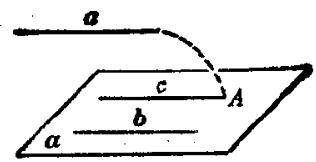
\includegraphics[width=5cm]{../pic/ltjh-ch1-20.png}
        \caption{}\label{fig:ltjh-1-20}
    \end{minipage}
    \qquad
    \begin{minipage}[b]{7cm}
        \centering
        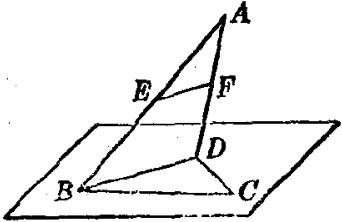
\includegraphics[width=5cm]{../pic/ltjh-ch1-21.png}
        \caption{}\label{fig:ltjh-1-21}
    \end{minipage}
\end{figure}

\liti 空间四边形相邻两边中点的连线,平行于经过另外两边的平面。

已知:空间四边形 $ABCD$ 中, $E$、$F$ 分別是 $AB$、$AD$ 的中点(图 \ref{fig:ltjh-1-21})。

求证: $EF \pingxing \text{平面} BCD$。

\zhengming 连线 $BD$。

\jiange
$\left.\begin{aligned}
    \left.\begin{aligned}
        AE = EB \\
        AF = FD
    \end{aligned}\right\} \tuichu & EF \pingxing BD \\
    & BD \subset \text{平面}\; BCD \\
    & EF \not \subset \text{平面}\; BCD
\end{aligned}\right\} \tuichu  EF \pingxing \text{平面}\; BCD \juhao$
\jiange

\begin{dingli}[直线和平面平行的性质定理][dl:zxhpmpx-xz]
    如果一条直线和一个平面平行,经过这条直线的平面和这个平面相交,那么这条直线就和交线平行。
\end{dingli}

已知: $a \pingxing \alpha$, $a \subset \beta$,  $\alpha \cap \beta = b$ (图 \ref{fig:ltjh-1-22})。

求证: $a \pingxing b$。

\zhengming $\because$ \quad $a \pingxing \alpha$,

$\therefore$ \quad $a$ 和 $\alpha$ 没有公共点。

又 $\because$ \quad $b \subset \alpha$,

$\therefore$ \quad $a$ 和 $b$ 没有公共点。

$a$ 和 $b$ 同在平面 $\beta$ 内,又没有公共点,

$\therefore$ \quad $a \pingxing b$。

\begin{figure}[htbp]
    \centering
    \begin{minipage}[b]{7cm}
        \centering
        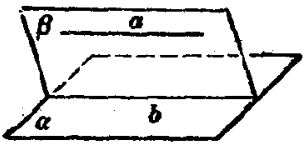
\includegraphics[width=5cm]{../pic/ltjh-ch1-22.png}
        \caption{}\label{fig:ltjh-1-22}
    \end{minipage}
    \qquad
    \begin{minipage}[b]{7cm}
        \centering
        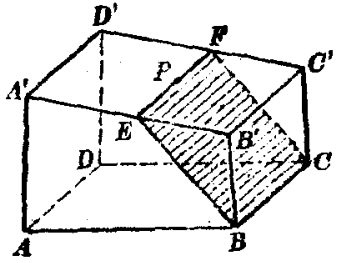
\includegraphics[width=5cm]{../pic/ltjh-ch1-23.png}
        \caption{}\label{fig:ltjh-1-23}
    \end{minipage}
\end{figure}

\liti 有一块木料如图 \ref{fig:ltjh-1-23},已知棱 $BC$ 平行于面 $A'C'$。
要经过木料表面 $A'B'C'D'$ 内的一点 $P$ 和棱 $BC$ 将木料锯开,应怎样画线?
所画的线和面 $AC$ 有什么关系?

\jie (1) $\because$ \quad $BC \pingxing \text{面}\;A'C'$,
面 $BC'$ 经过 $BC$ 和面 $A'C'$ 交于 $B'C'$,

$\therefore$ \quad $BC \pingxing B'C'$。

经过点 $P$, 在面 $A'C'$ 上画线段 $EF \pingxing B'C'$,
根据\nameref{gl:zxpx},$EF \pingxing BC$。

$\therefore$ \quad $EF \subset \text{平面}\;BF$, $BC \subset \text{平面}\;BF$。
连结 $BE$ 和 $CF$, $BE$、$CF$ 和 $EF$ 就是所要画的线。

(2) $\because$ \quad $EF \pingxing BC$,根据\hyperref[dl:zxhpmpx-pd]{判定定理},
则 $EF \pingxing \text{面}\; AC$;
$BE$、$CF$ 显然都和面 $AC$ 相交。


\begin{lianxi}

\xiaoti{使一块矩形木板 $ABCD$ 的一边 $AB$ 靠紧桌面 $\alpha$,并绕 $AB$ 转动。
    $AB$ 的对边 $CD$ 在各个位置时,是不是都和桌面 $\alpha$ 平行?为什么?
}

\xiaoti{长方体的各个面都是矩形,说明长方体每一个面的各边及对角线为什么都和相对的面平行。}


\xiaoti{图 \ref{fig:ltjh-1-23} 中,如果 $AD \pingxing BC$, $BC \pingxing \text{面}\; A'C'$,
    那么, $AD$ 和面 $BC'$、面 $BF$、面 $A'C'$ 都有怎样的位置关系。为什么?
}

\end{lianxi}

